% +------------------------------------------------------------------------+
% | CGAL User Manual: 
% +------------------------------------------------------------------------+
% |
% | 28.05.2008   Peter Hachenberger
% | 
\RCSdef{\ConvexDecomposition3Rev}{$Id$}
\RCSdefDate{\ConvexDecomposition3Date}{$Date$}
% +------------------------------------------------------------------------+

\ccParDims

\ccUserChapter{Convex Decomposition of Polyhedra \label{chapterConvexDecomposition3}}
\ccChapterRelease{\ConvexDecomposition3Rev. \ \ConvexDecomposition3Date}
\ccChapterAuthor{Peter Hachenberger}


\begin{ccPkgDescription}{3D Convex Hulls\label{Pkg:ConvexHull3}}
\ccPkgHowToCiteCgal{cgal:hs-ch3-07}
\ccPkgSummary{This package provides functions 
for computing convex hulls in three dimensions as well as functions
for checking if sets of points are strongly convex are not. One can
compute the convex hull of a set of points in three dimensions in one
of three ways: using a static algorithm, using an incremental
construction algorithm, or using a triangulation to get a fully
dynamic computation.}

\ccPkgDependsOn{All algorithms produce as output a \ccRef[3D Polyhedron]{Pkg:Polyhedron}. 
                The dynamic algorithms depend on \ccRef[3D Triangulations]{Pkg:Triangulation3}}
\ccPkgIntroducedInCGAL{1.1}
\ccPkgLicense{\ccLicenseQPL}
\ccPkgIllustration{Convex_hull_3/bunny.png}{Convex_hull_3/bunny.png}
\end{ccPkgDescription}


% +------------------------------------------------------------------------+
\section{Introduction}

For many applications on non-convex polyhedra, there are efficient
solutions that first decompose the polyhedron into convex pieces. As
an example, the Minkowski sum of two polyhedra can be computed by
decomposing both polyhedra into convex pieces, compute pair-wise
Minkowski sums of the convex pieces, and unite the pair-wise sums.

While it is desirable to have a decomposition into a minimum number of
pieces, this problem is know to be NP-hard~\cite{c-cpplb-84}. Our
implementation decomposes a Nef polyhedron $N$ into $O(r^2)$ convex
pieces, where $r$ is the number of edges, which have two adjacent
facets that span an angle of more than 180 degrees with respect to the
interior of the polyhedron. Those edges are also called reflex edges.
The bound of $O(r^2)$ convex pieces is worst-case
optimal~\cite{c-cpplb-84}.

\begin{figure}[h]
  \begin{ccTexOnly}
    \begin{center}
      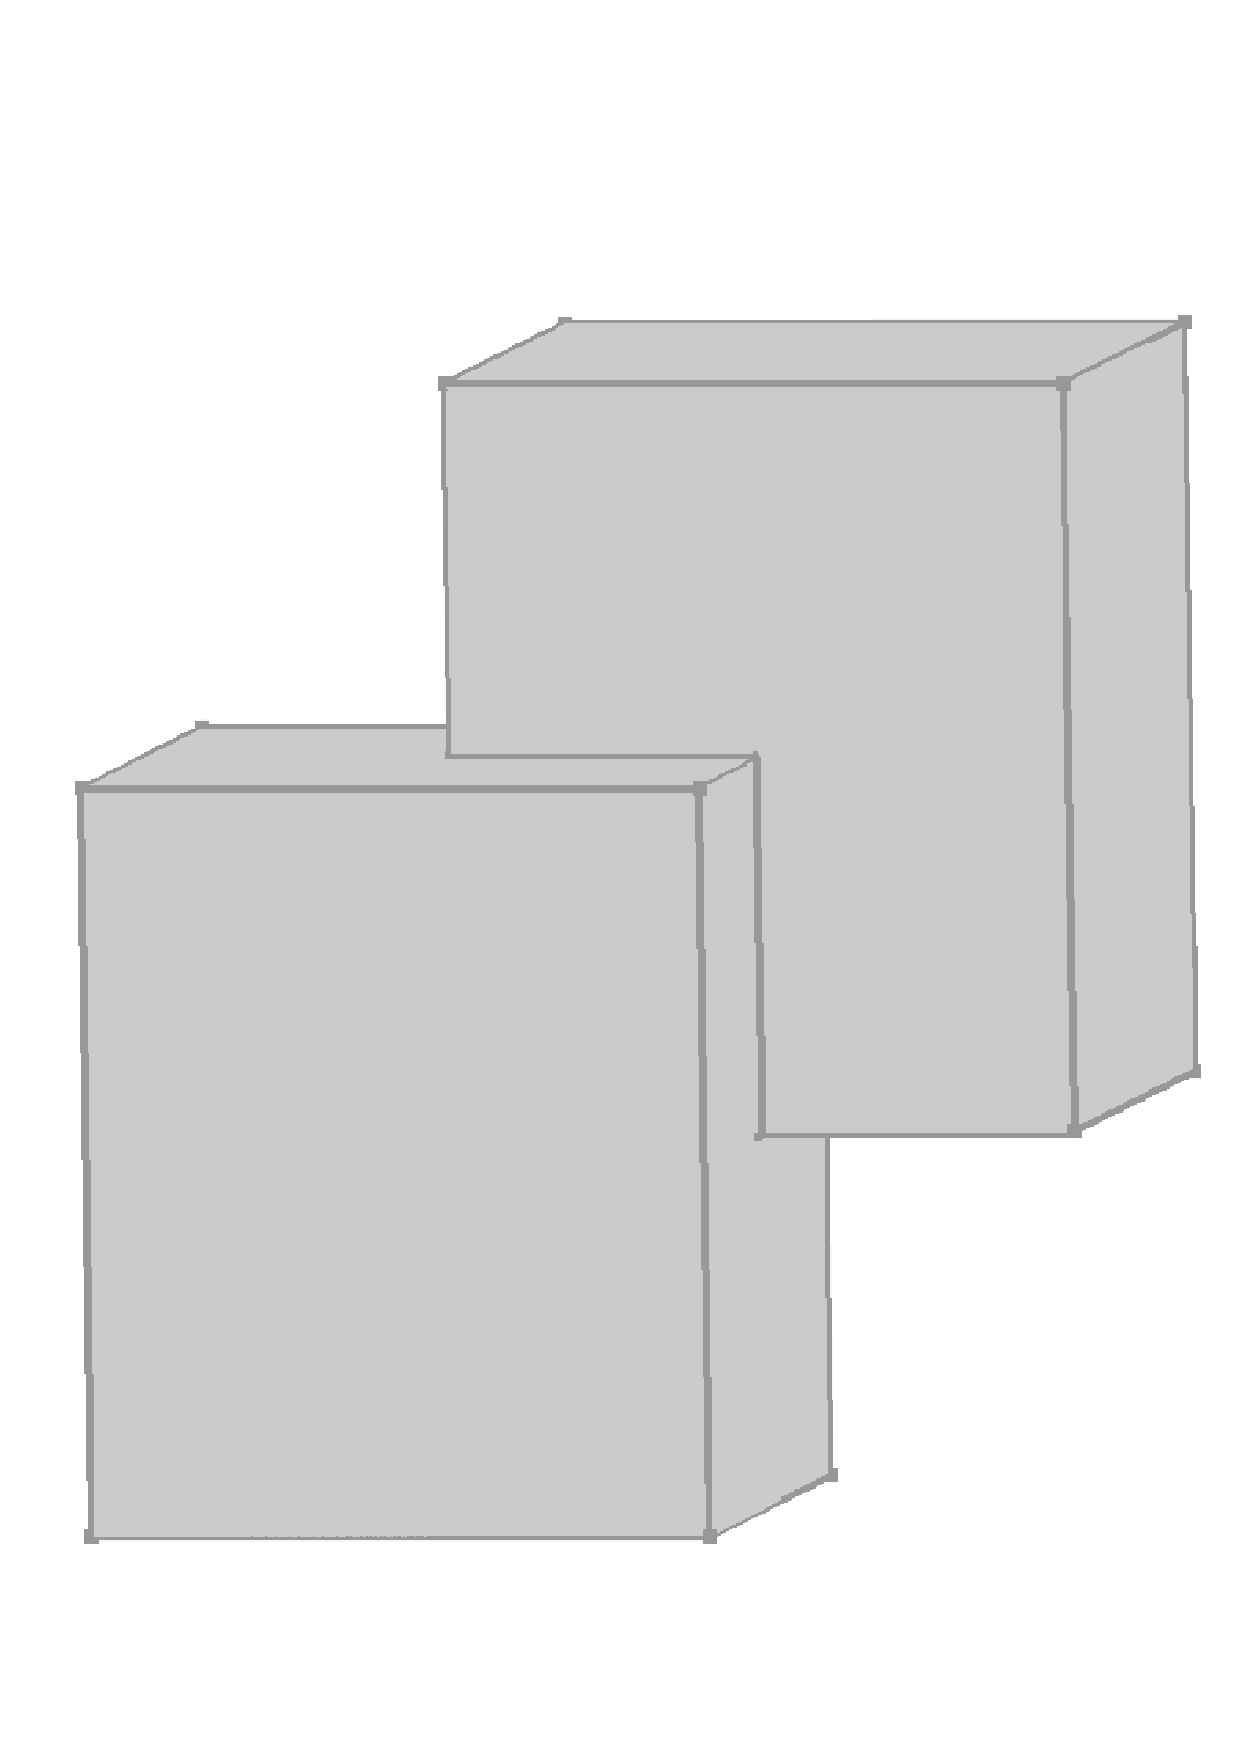
\includegraphics[width=0.245\textwidth]{Convex_decomposition_3/fig/two_cubes} \hspace{4mm}
      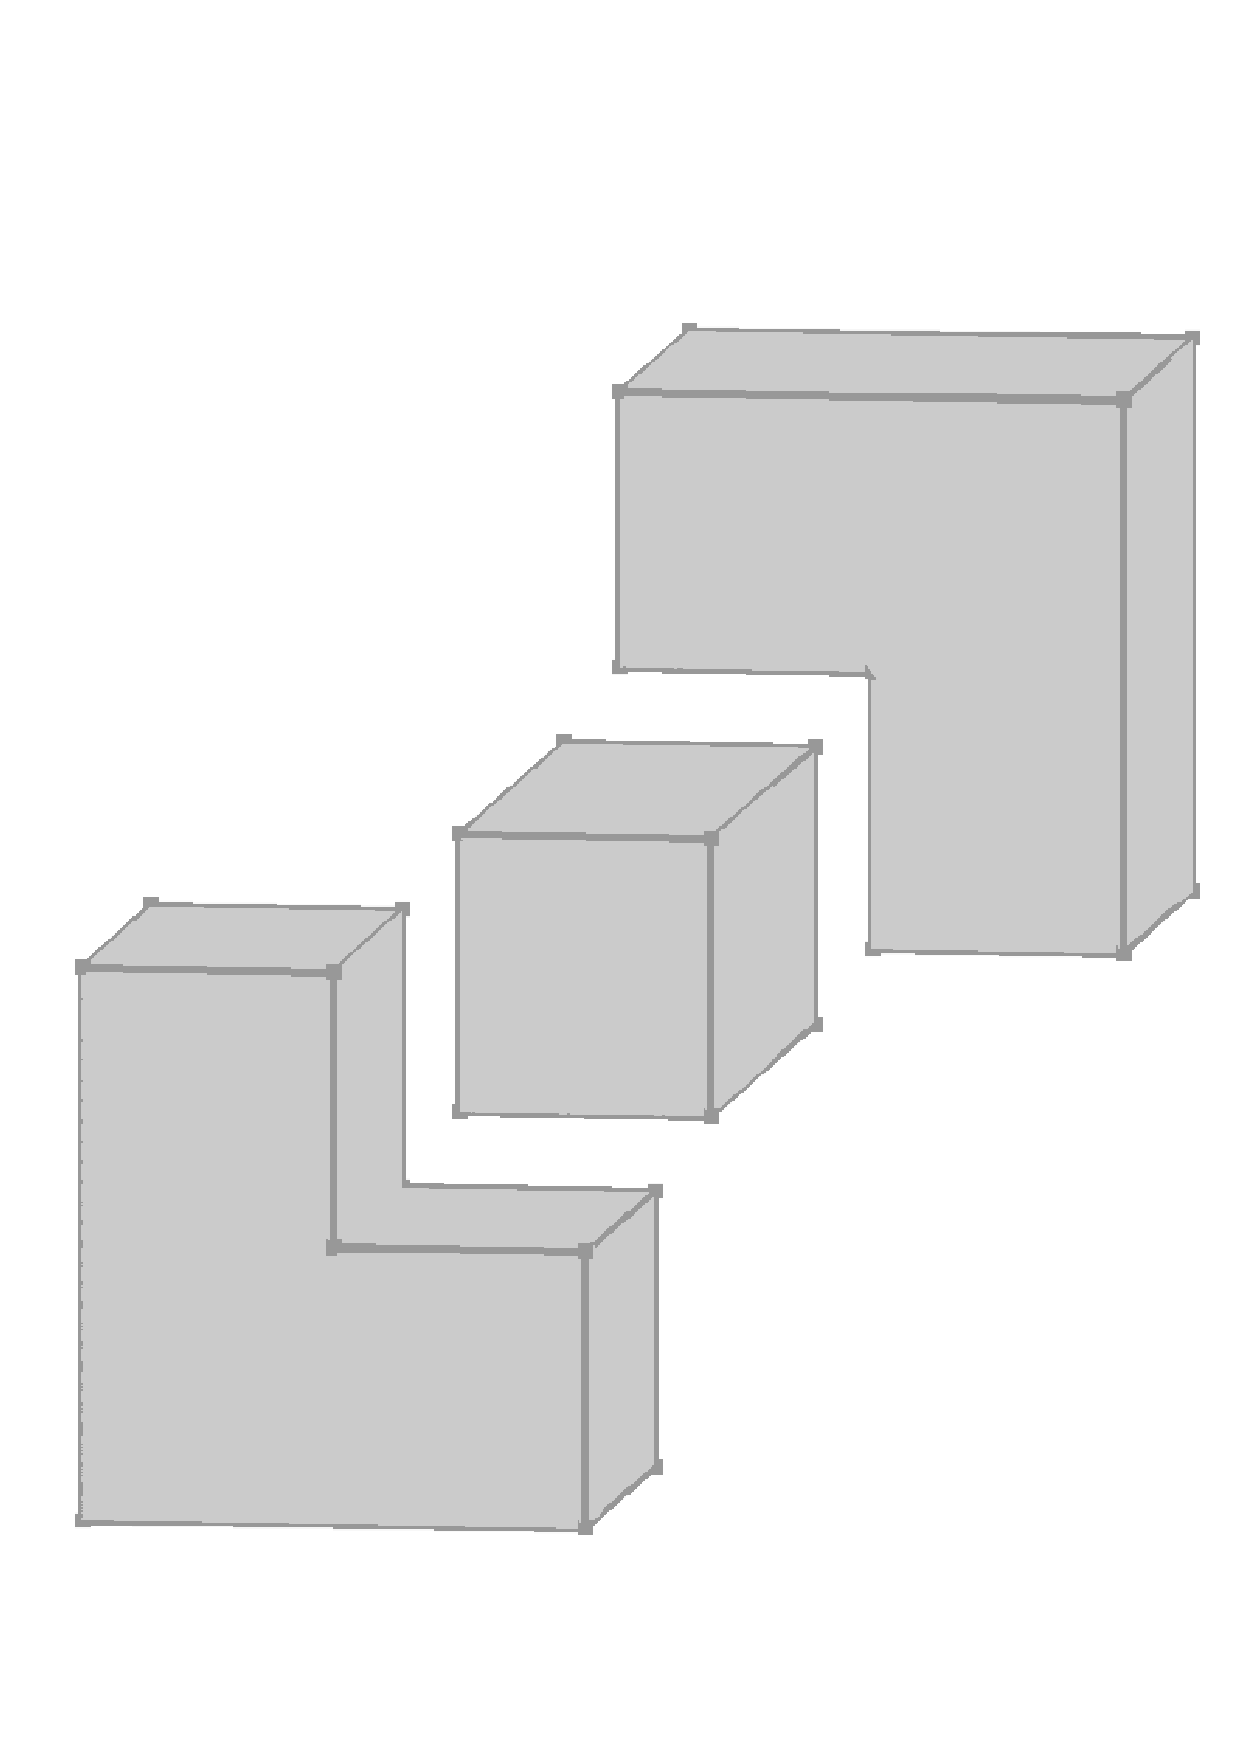
\includegraphics[width=0.25\textwidth]{Convex_decomposition_3/fig/two_cubes_cylindrical} \hspace{1mm}
      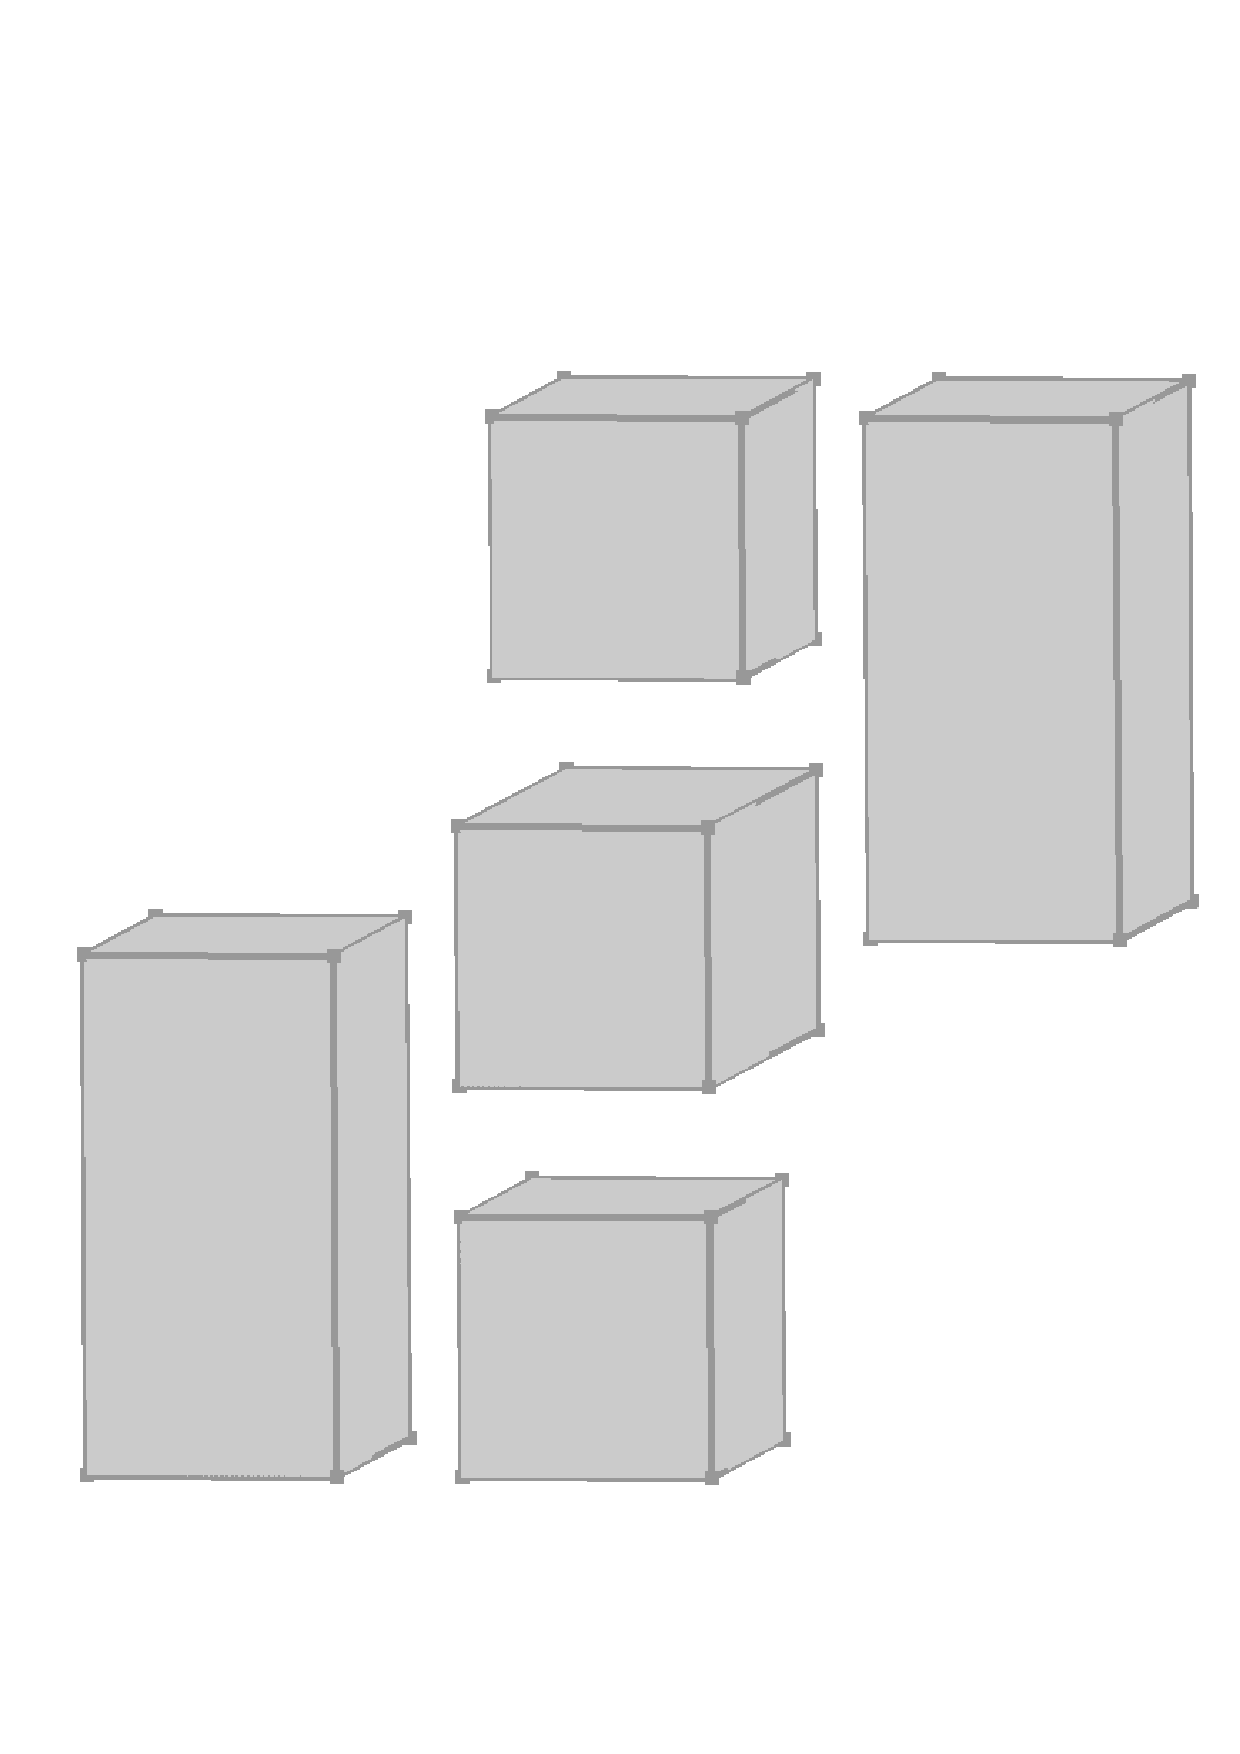
\includegraphics[width=0.27\textwidth]{Convex_decomposition_3/fig/two_cubes_vertical}
    \end{center}
  \end{ccTexOnly}
  \begin{ccHtmlOnly}
    <p><center>
    <img src="./fig/two_cubes.gif" border=0 alt="decomposition
    example">
    <img src="./fig/two_cubes_cylindrical.gif" border=0 alt="decomposition
    after first step">
    <img src="./fig/two_cubes_vertical.gif" border=0 alt="final decomposition">
    </center>
  \end{ccHtmlOnly}
  \caption{Vertical decomposition based on the insertion of walls 
	   (viewed from the top). Left: Non-convex polyhedron. Middle:
	   Non-vertical reflex edges have been resolved. Right: Vertical
           reflex edges have been resolved. The cells are convex.}
  \label{fig:verticalDecomposition}
\end{figure}

Our decomposition runs in two steps. In the first step, each
non-vertical reflex edge $e$ is resolved by insertion of vertical
facets $W(e)$ through $e$. In the second step, we do the same with the
vertical reflex edges. Figure~\ref{fig:verticalDecomposition}
illustrates the two steps.

The worst-case running time of our implementation is
$O(n^2r^4\sqrt[3]{nr^2}\log{nr})$, where $n$ is the complexity of the
polyhedron and $r$ is the number of reflex edges. But this running
time is very pessimistic. Assuming that every inserted facet has
complexity $O(n)$ and that ray shooting queries run in logarithmic
time, the running time is $O(nr^2\log{nr})$.

At the moment our implementation is restricted to the decomposition of
bounded polyhedra. An extension to unbounded polyhedra is planned.

% +------------------------------------------------------------------------+
\section{Interface and Usage}

A \ccc{Nef_polyhedron_3} represents a subdivision of the
three-dimensional space into vertices, edges, facets, and
volumes. Each of these items contains set-selection mark, which
indicates whether the item belongs to the represented point set or
not. The represented polyhedron is the union of the point sets
represented by the selected items. As an example, a cube is
represented by 8 vertices, 12 edges, 6 facets, and 2 volumes, where
one volume represents the interior of the cube and the other the
volume outside of the cube. All of these items are selected, except
for outer volume.  Read the chapter on 3D Boolean operations on Nef
polyhedra for more details~\ref{chapterNef3}.

The function \ccc{convex_decomposition_3} takes one
\ccc{Nef_polyhedron_3} as input an inserts additional facets into the
selected volumes. These additional facets are also selected and
therefore redundant for the representation of the polyhedron. If some
of these facets split a volume into two parts, each of the two volumes
is represented by a separate volume item. The insertion of facets
stops when all the selected volumes are convex. The modified
polyhedron is the result of the function
\ccc{convex_decomposition_3}. Note that the function 
\ccc{convex_decomposition_3} is restricted to standard kernels. 
The extended kernels, which allow the representation of polyhedra with
an infinite boundary (e.g. halfspaces) only add further unbounded
polyhedra to the domain of representable polyhedra. Using a standard
kernel, unbounded polyhedra can be identified by the selected outer
volume. In such a case, we ignore the outer volume in the
decomposition process.

The convex pieces of the modified polyhedron can be accessed by
traversing $N$, as described in Section~\ref{subsectionNef_3ShellExploration} of the
user manual pages of the Nef polyhedron, or by converting
them into separate Nef polyhedra, as illustrated by the example code.

\ccIncludeExampleCode{Convex_decomposition_3/list_of_convex_parts.cpp}
